\documentclass[12pt]{article}

\usepackage[spanish]{babel}
\usepackage{hyperref}
\usepackage{graphicx}
\usepackage{listings}
\usepackage{color}
\usepackage{multicol}
\usepackage{amssymb}
\usepackage{enumitem}
\usepackage{here}
\usepackage{dsfont}
\usepackage{amsmath}
\usepackage{tipa}
\usepackage{float}
\spanishdecimal{.}

\title{Matemáticas para las Ciencias Aplicadas I}
\title{
	Tercera Lista de Problemas \\
	\textbf{Tercera  Parte} \\
	\vspace{1ex}
	\large Matemáticas para las Ciencias Aplicadas I \\
	Facultad de Ciencias, UNAM}

\date{\today}

\author{Flores Morán Julieta Melina \\ Zarco Romero José Antonio}

\begin{document}

\maketitle

%% De la sección 4.4: ejercicios 48 y 53
%% De la sección 4.5: ejercicios 14, 47, 64 y 65
%% De la sección 4.6: ejercicios 24 y 40
%% De la sección 4.7: ejercicios 18 y 34

%%  -----------------------------------------------------------------------------------------------------------------------------------------------------------------------------------------------------------------------------
\section{Sección 4.4 \\ Máximos Y Mínimos Absolutos}
% 48 -------------------------------------------------------------------------------------------------------------
\subsection{Ejercicio 48} Zarco Romero José Antonio \\

Demuestre que $\cos{x} \geq 1-(x^2 /2)$ para todo $x$ en el intervalo $[0, 2\pi]$. \\

Una manera de demostrar que $\cos{x} \geq 1-(x^2 /2)$ para todo $x$ en el intervalo $[0, 2\pi]$ es demostrar que $0 \leq \cos{x}-[1-(x^2 /2)]$, es decir $0 \leq \frac{x^2}{2}+\cos{x}-1$, para todo $x$ en el intervalo dado; y una forma de demostrar esta última desigualdad es demostrar que el valor mínimo absoluto de $y=\frac{x^2}{2}+\cos{x}-1$ en el intervalo no es negativo. Para demostrar esto, tenemos que la continuidad de $f$ junto con el hecho de que
\[
\lim_{x \to 0} \frac{x^2}{2}+\cos{x}-1 = \frac{0^2}{2}+\cos{0}-1 = 0+1-1=0
\]
es finito y permite la posibilidad de que $f$ tenga un mínimo absoluto en $[0, 2\pi]$. Si es así, tendría que ocurrir en un punto crítico de $f$, por lo que consideramos
\[
f'(x) = x-\sin{x}
\]
dicha derivada es $\geq 0$ para todo valor de $x$ en el intervalo $[0, 2\pi]$
\[
f'(0)=0-\sin{0}=0-0=0
\]
$\therefore \cos{x} \geq 1-(x^2 /2)$ para todo $x$ en el intervalo $[0, 2\pi]$.
\begin{flushright}
  $\blacksquare$
\end{flushright}

% 53 -------------------------------------------------------------------------------------------------------------
\subsection{Ejercicio 53} Zarco Romero José Antonio \\

Supongamos que las ecuaciones de movimiento de un avión de papel durante los primeros 12 segundos de vuelo son
\begin{align*}
  x=t-2\sin{t} && y=2-2\cos{t} && (0\leq t\leq 12)
\end{align*}

¿Cuáles son los puntos más alto y más bajo de la trayectoria, y cuándo está el avión en esos puntos? \\

A fin de conocer los extremos absolutos, debemos encontrar $y'(t)$, esto es
\[
y'(t)=2\sin{t}
\]

Sabemos, por el comportamiento de $\sin{t}$, que $y'(t)=0$ cuando $t$ es múltiplo de $\pi$, es decir $t=k\pi$ donde $k$ es un entero entre 0 y 3, inclusive.

Evaluando $y$ en los siguientes puntos, obtenemos que
\begin{align*}
  y(0)
  &= 2-2\cos{0} = 2-2 = 0 \\
  y(\pi)
  &= 2-2\cos{\pi} = 2+2 = 4\\
  y(2\pi)
  &= 2-2\cos{2\pi} = 2-2 = 0\\
  y(3\pi)
  &= 2-2\cos{3\pi} =  2+2 = 4
\end{align*}

de lo cual concluimos que el mínimo absoluto de $y$ en $0\leq t\leq 12$ es 0, que ocurre en $t=0,2\pi$, y el máximo absoluto de $y$ en $0\leq t\leq 12$ es 4, que ocurre en $t = \pi,3\pi$.

$\therefore $ Los puntos más altos de trayectoria son $(\pi,4)$ y $(3\pi,4)$. A su vez, los puntos más bajos de trayectoria son $(0,0)$ y $(2\pi,0)$.

%%  -----------------------------------------------------------------------------------------------------------------------------------------------------------------------------------------------------------------------------
\section{Sección 4.5 \\ Problemas De Máximos Y Mínimos Aplicados}
% 14 -------------------------------------------------------------------------------------------------------------
\subsection{Ejercicio 14} Zarco Romero José Antonio \\

Un alambre de 12 pulgadas de largo se puede doblar en un círculo, doblar en un cuadrado o cortar en dos pedazos para formar un círculo y un cuadrado. ¿Cuánto alambre se debe usar para el círculo si el área total encerrada por las figura(s) debe ser (a) un máximo (b) un mínimo? \\

Sea
\begin{itemize}
\item $A= $ área total encerrada por las figuras $(in^2)$
\item $r= $ radio del círculo $(in)$
\item $l= $ longitud de los lados del cuadrado $(in)$
\end{itemize}

Como la fórmula para el área es la suma de ambas figuras, tenemos
\[
A=\pi r^2 + l^2
\]

Sabemos también que el perímetro del círculo está dado por la fórmula $x=2\pi r$, por lo que $r=\frac{x}{2\pi}$. Análogamente el perímetro del cuadrado está dado por la fórmula $y=4l$, por lo que $l=\frac{y}{4}$. Al sustituir estos valores en la fórmula del área tenemos
\begin{align*}
  A
  = \pi \left( \frac{x}{2\pi} \right)^2 + \left( \frac{y}{4} \right)^2
  = \frac{x^2}{4\pi}+\frac{y^2}{16}
\end{align*}

Como el largo del alambre es de 12 pulgadas, las variables $x$ y $y$ están relacionadas mediante la ecuación
\begin{align*}
  x+y=12 \text{, así } y=12-x
\end{align*}

Sustituyendo en la ecuación del área tenemos que
\begin{align*}
  A
  &= \frac{x^2}{4\pi}+\frac{(12-x)^2}{16} \\
  &= \frac{x^2}{4\pi}+\frac{144-24x+x^2}{16} \\
  &= \frac{4x^2+\pi x^2-24\pi x +144\pi}{16\pi} \\
  &= \frac{4x^2+\pi x^2}{16\pi} - \frac{24\pi x }{16\pi} + \frac{+144\pi}{16\pi}\\
  &= \frac{\pi + 4}{16\pi}x^2-\frac{3}{2}x+9
\end{align*}

que expresa $A$ en términos de $x$ únicamente. Debido a que $x$ representa una longitud, no puede ser negativa y debido a que no puede exceder la longitud del alambre de 12 pulgadas; la variable $x$ debe satisfacer

\[
0 \leq x \leq 12
\]

Así, hemos reducido el problema al de encontrar el valor (o valores) de $x$ en $[0, 12]$, para el cual $A$ es máximo/mínimo. Como $A$ es un polinomio en $x$, es continuo en $[0, 12]$, por lo que el máximo/mínimo debe ocurrir en un punto final de este intervalo o en un punto crítico.

Procedemos ahora a diferenciar $A$ con respecto a $x$
\begin{align*}
  \frac{dA}{dx}
  &= \frac{\pi+4}{8\pi}x-\frac{3}{2}
\end{align*}

Calculando $dA/dx = 0$ obtenemos
\begin{align*}
  \frac{\pi+4}{8\pi}x-\frac{3}{2}
  &= 0\\
  \frac{\pi+4}{8\pi}x
  &=\frac{3}{2}\\
  x
  &=\frac{12\pi}{\pi+4}\\
\end{align*}

Evaluando $A$ en los siguientes puntos, obtenemos que
\begin{align*}
  A(0)
  &= \frac{\pi + 4}{16\pi}(0)^2-\frac{3}{2}(0)+9=9\\
  A\left(\frac{12\pi}{\pi+4}\right)
  &= \frac{\pi + 4}{16\pi}\left(\frac{12\pi}{\pi+4}\right)^2-\frac{3}{2}\left(\frac{12\pi}{\pi+4}\right)+9 \\
  &= \frac{9\pi}{x+4}-\frac{18\pi}{\pi+4}+9 \\
  &= \frac{-9\pi+9\pi+36}{\pi+4} \\
  &= \frac{36}{\pi+4}\\
  A(12)
  &= \frac{\pi + 4}{16\pi}(12)^2-\frac{3}{2}(12)+9\\
  &= \frac{\pi + 4}{16\pi}(144)-9\\
  &= \frac{\pi + 4}{\pi}(9)-9\\
  &= \frac{9\pi + 36-9\pi}{\pi}\\
  &= \frac{36}{\pi}
\end{align*}

$\therefore $ El alambre que debe usarse para el círculo si el área total encerrada por las figuras debe ser un \textbf{máximo} es $x=12$, y $x=\frac{12\pi}{\pi+4}$ si debe ser un \textbf{mínimo}.

% 47 -------------------------------------------------------------------------------------------------------------
\subsection{Ejercicio 47} Flores Morán Julieta Melina \\

Un trapezoide está inscrito en un semicírculo de radio 2 de modo que un lado está a lo largo del diámetro (Figura Ex-47). Encuentra el área máxima posible para el trapezoide. [\textit{Sugerencia}: Exprese el área del trapezoide en términos de $\theta$.]\\
\begin{figure}[H]
\centering
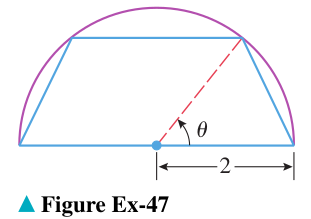
\includegraphics[width=0.4\textwidth]{../img/img_Lista3/3_47.png}
\end{figure}
La cantidad a maximizar es el área del trapecio, cuya fórmula general es $A= \frac{B+b}{2}h$. Entonces las variables cuyos valores necesitamos expresar con la información que tenemos son:\\
- Base mayor (B): La base mayor del trapecio siempre será el diámetro del semicírculo que es $D=2r$, es decir $D=2(2) = 4$. Así  que (B = 4).\\
- Altura (h) : Hay que notar que se puede construir un triángulo rectángulo con el ángulo donde la hipotenusa es el radio, el cateto adyacente parte de la Base mayor y el cateto opuesto la altura del trapecio. Así que la altura la podemos entender en términos del seno. Considerando que $\sin{\theta}\frac{co}{h}$, podemos despejar el cateto opuesto $co = h\sin{\theta}$. Siendo el cateto opuesto la altura y la hipotenusa 2. $h = 2\sin{\theta}$.\\
- Base menor (b): Siguiendo con el triángulo anteriormente descrito, la base menor equivaldrá al doble de lo que valga el cateto adyacente de nuestro triángulo rectángulo. El cateto adyacente se da fácilmente en términos del coseno ya que $\cos{\theta} = \frac{ca}{h}$ así que se puede despejar el cateto como $ca = h\cos{\theta}$. Siendo que h es 2 $ca = 2\cos{\theta}$. Y como habíamos mencionado, la base menor será el doble de este valor, por lo que $b = 4\cos{\theta}$.\\
Con estas sustituciones encontramos la función a maximizar, $A(\theta) = \frac{4+4\cos{\theta}}{2}\cdot( 2\sin{\theta}) $, en un intervalo donde $0 \leq \theta \leq \frac{\pi}{2}$ ya que en $\pi/2$ la base menor es 0 pero después negativa, y no tenemos longitudes de este tipo.
Para encontrar el máximo en el intervalo $[0,\pi /2 ]$sabemos que se puede encontrar en los extremos o en puntos críticos de esta función. Así que encontremos estos puntos derivando.
\begin{align*}
  A''(\theta)
  &= \frac{d}{d\theta} \left[  \frac{1}{2}(4+4\cos{\theta})( 2\sin{\theta}) \right]\\
  &= \frac{1}{2}  \frac{d}{d\theta}  \left[ (4+4\cos{\theta})( 2\sin{\theta}) \right]\\
  &= \frac{1}{2}   \left[ (4+4\cos{\theta}) \frac{d}{d\theta}  ( 2\sin{\theta}) + ( 2\sin{\theta}) \frac{d}{d\theta}  (4+4\cos{\theta})  \right]\\
  &= \frac{1}{2}   \left[ (4+4\cos{\theta}) ( 2\cos{\theta}) - ( 2\sin{\theta})  (4\sen{\theta})  \right]\\
  &= \frac{1}{2}   \left[  8\cos{\theta} + 8\cos^{2}\theta   - 8\sin^{2}\theta   \right] \\
  &= \frac{8}{2}   \left[  \cos{\theta} + \cos^{2}\theta   - \sin^{2}\theta   \right] \\
  &= 4   \left[  \cos{\theta} + \cos^{2}\theta   - \sin^{2}\theta   \right] \\
  &= 4   \left[  \cos{\theta} + \cos^{2}\theta   -  [1-cos^{2}\theta]   \right] \\
  &= 4   \left[  \cos{\theta} + \cos^{2}\theta   - 1 + cos^{2}\theta   \right] \\
  &= 4   (2cos\theta-1)(cos\theta+1) \\ 
\end{align*}
Ahora, los puntos críticos serán cuando $2cos\theta-1=0$ y $cos\theta+1=0$.
\[
2cos\theta-1=0 
\]
\[
2cos\theta=1 
\]
\[
cos\theta=\frac{1}{2} 
\]
\[
\theta=cos^-1 \left(\frac{1}{2}  \right) = \frac{\pi}{3}
\]
y
\[
cos\theta+1 =0
\]
\[
cos\theta =-1
\]
\[
\theta =cos^{-1}(-1) = \pi
\]
Pero este último esta fuera del rango, así que el punto crítico será $\frac{\pi}{3}$.\\
Ahora hay que evaluar los extremos, es decir, $0$,  $\frac{\pi}{3}$ y $\frac{\pi}{2}$.\\
\[
A(0)= \frac{4+4\cos{0}}{2}\cdot( 2\sin{0}) = 0
\]
\[
A(\frac{\pi}{3})= \frac{4+4\cos{\frac{\pi}{3}}}{2}\cdot( 2\sin{\frac{\pi}{3}})= 3 \sqrt{3}
\]
\[
A(\frac{\pi}{2})= \frac{4+4\cos{\frac{\pi}{2}}}{2}\cdot( 2\sin{\frac{\pi}{2}}) = 4
\]
$\therefore$ El máximo $(\frac{\pi}{3}, 3 \sqrt{3} )$ y el área máxima es $3 \sqrt{3}$.

\begin{figure}[H]
\centering
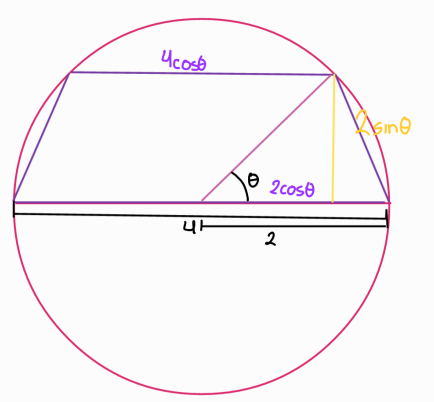
\includegraphics[width=0.4\textwidth]{../img/img_Lista3/trapecio.png}
\end{figure}

% 64 -------------------------------------------------------------------------------------------------------------
\subsection{Ejercicio 64} Zarco Romero José Antonio \\

\textit{\textbf{El principio de Fermat}} en óptica establece que la luz que viaja de un punto a otro sigue aquel camino cuyo tiempo total de viaje es mínimo. En un medio uniforme, los caminos de ``tiempo mínimo'' y ``distancia más corta'' resultan ser los mismos, de modo que la luz, si no hay obstáculos, viaja en línea recta. Supongamos que tenemos una fuente de luz, un espejo plano y un observador en un medio uniforme. Si un rayo de luz sale de la fuente, rebota en el espejo y viaja hasta el observador, entonces su trayectoria constará de dos segmentos de línea, como se muestra en la Figura Ex-64. Según el principio de Fermat, el camino será tal que el tiempo total de viaje $t$ sea mínimo o, dado que el medio es uniforme, el camino será tal que la distancia total recorrida de $A$ a $P$ y a $B$ sea lo más pequeña posible. Suponiendo que el mínimo ocurre cuando $dt/dx = 0$, demuestre que el rayo de luz incidirá en el espejo en el punto $P$ donde el ``ángulo de incidencia'' $\theta_1$ es igual al ``ángulo de reflexión'' $\theta_2$.
\begin{figure}[H]
\centering
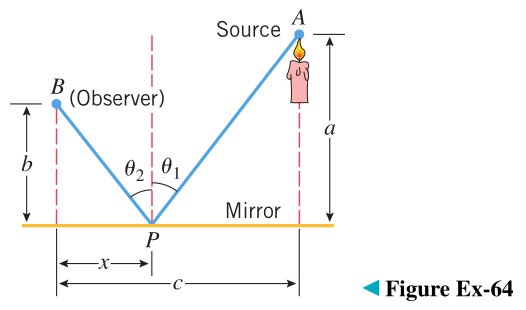
\includegraphics[width=0.7\textwidth]{../img/img_Lista3/3_64.png}
\end{figure}

Sea
\begin{itemize}
\item $t= $ tiempo total de viaje
\item $d= $ distancia total de $\overleftrightarrow{AP}+\overleftrightarrow{PB}$
\item $v= $ velocidad de la luz en el medio uniforme
\end{itemize}

La fórmula para calcular el tiempo es 
\[
t=\frac{d}{v}
\]

donde $d=\overleftrightarrow{AP}+\overleftrightarrow{PB}=\sqrt{x^2+b^2}+\sqrt{(c-x)^2+a^2}$. Entonces,
\[
t=\frac{1}{v}\left( \sqrt{x^2+b^2}+\sqrt{(c-x)^2+a^2} \right)
\]

Diferenciando $t$ respecto a $x$, tenemos
\begin{align*}
  \frac{dt}{dx}
  &=\frac{1}{v}\left[ \frac{x}{\sqrt{x^2+b^2}}-\frac{c-x}{\sqrt{(c-x)^2+a^2}} \right]
\end{align*}

Calculando $dt/dx = 0$ obtenemos
\begin{align*}
  \frac{1}{v}\left[ \frac{x}{\sqrt{x^2+b^2}}-\frac{c-x}{\sqrt{(c-x)^2+a^2}} \right]
  &= 0 \\
  \frac{x}{\sqrt{x^2+b^2}}-\frac{c-x}{\sqrt{(c-x)^2+a^2}}
  &= 0 \\
  \frac{x}{\sqrt{x^2+b^2}}
  &=\frac{c-x}{\sqrt{(c-x)^2+a^2}}
\end{align*}

Observando la Figura Ex-64, nótese que $\sin{\theta_2}=\frac{x}{\sqrt{x^2+b^2}}$ y $\sin{\theta_1}=\frac{c-x}{\sqrt{(c-x)^2+a^2}}$

Por tanto, $dt/dx = 0$ cuando $\sin{\theta_2}=\sin{\theta_1}$, entonces $\theta_2 = \theta_1$. \\

$\therefore $ El ``ángulo de incidencia'' $\theta_1$ es igual al ``ángulo de reflexión'' $\theta_2$ cuando el rayo de luz incida en el espejo en el punto $P$.

\begin{flushright}
  $\blacksquare$
\end{flushright}

% 65 -------------------------------------------------------------------------------------------------------------
\subsection{Ejercicio 65} Flores Morán Julieta Melina \\

El principio de Fermat (Ejercicio 64) también explica por qué los rayos de luz que viajan entre el aire y el agua se curvan (refracción). Imagine que tenemos dos medios uniformes (como aire y agua) y un rayo de luz que viaja desde una fuente $A$ en un medio hasta un observador $B$ en el otro medio (Figura Ex-65). Se sabe que la luz viaja a una velocidad constante en un medio uniforme, pero más lenta en un medio denso (como el agua) que en un medio fino (como el aire). En consecuencia, el camino de menor tiempo de A a B no es necesariamente una línea recta, sino más bien un camino de línea discontinua de $A$ a $P$ a $B$ que permite a la luz aprovechar al máximo su mayor velocidad a través del medio delgado. \textit{\textbf{La ley de refracción de Snell}} establece que la trayectoria del rayo de luz será tal que
\[
\frac{\sin{\theta_1}}{v_1}=\frac{\sin{\theta_2}}{v_2}
\]
donde $v_1$ es la velocidad de la luz en el primer medio, $v_2$ es la velocidad de la luz en el segundo medio y $\theta_1$ y $\theta_2$ son los ángulos que se muestran en la figura Ex-65. Demuestre que esto se deriva del supuesto de que la trayectoria del tiempo mínimo ocurre cuando $dt /dx = 0$.\\
\begin{figure}[H]
\centering
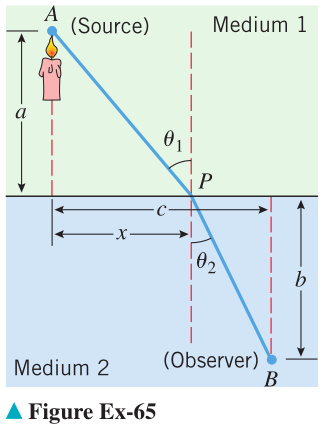
\includegraphics[width=0.4\textwidth]{../img/img_Lista3/3_65.png}
\end{figure}
La fórmula a minimizar es la del tiempo, y sabemos que el tiempo total debe ser la suma del tiempo que tarda en viajar por un medio y el tiempo que tarda en el otro. \\
$T_t$ = Tiempo de A-P + Tiempo de P-B\\
Sabemos que en general $t = \frac{d}{v}$.
Así que para el primer tramo AP que transcurre en un medio en el que la luz tiene una velocidad $v_1$. Necesitamos conocer la distancia recorrida. Por la imagen podemos notar que la distancia recorrida es la hipotenusa de un triángulo rectángulo donde el cateto adyacente a $\theta_1$ es a y el opuesto x. Por lo tanto el valor de $AP= \sqrt{a^2+x^2}$. 
\[
t_{AP}= \frac{\sqrt{a^2+x^2}}{v_1}
\]
Para el segundo tramo seguimos el mismo razonamiento, en el segundo medio la luz tiene una velocidad $v_2$ y por la imagen podemos identificar que el cateto adyacente a $\theta_2$ es b y el opuesto es c-x por lo que $PB= \sqrt{b^2 + (c-x)^2}$.
\[
t_{PB}= \frac{\sqrt{b^2 + (c-x)^2}}{v_2}
\]
Por lo tanto, podemos remplazar en la fórmula propuesta y obtener:
\[
T_t= \frac{\sqrt{a^2+x^2}}{v_1} +  \frac{\sqrt{b^2 + (c-x)^2}}{v_2}
\]
Ahora para encontrar el punto donde $\frac{dt}{dx}=0$ hay que derivar esta formula.
\begin{align*}
  T_t'
  &=  \frac{d}{dx} \frac{\sqrt{a^2+x^2}}{v_1} +  \frac{d}{dt} \frac{\sqrt{b^2 + (c-x)^2}}{v_2}\\
  &= \frac{1}{v_1} \frac{d}{dx} (a^2+x^2)^{1/2}+\frac{1}{v_2} \frac{d}{dx}  (b^2 +(c-x)^2)^{1/2}\\
  &= \frac{1}{v_1} \frac{1}{2} (a^2+x^2)^{-1/2} \cdot 2x + \frac{1}{v_2} \frac{1}{2}  (b^2 +(c-x)^2)^{-1/2} \cdot 2(c-x) \cdot -1\\
  &= \frac{2x}{2v_1  \cdot (a^{2} + x^{2})^{1/2}}  - \frac{2(c-x)}{2v_2\cdot (b^2 +(c-x)^2)^{1/2} }\\
  &= \frac{x}{v_1  \cdot \sqrt{a^{2} + x^{2}}}  - \frac{c-x}{v_2\cdot \sqrt {b^2 +(c-x)^2)} } \\
  &= \frac{1}{v_1}\frac{x}{  \sqrt{a^{2} + x^{2}}}  - \frac{1}{v_2}\frac{c-x}{ \sqrt {b^2 +(c-x)^2)} } 
\end{align*}
Es evidente que la derivada valdrá 0 cuando ocurra que:
\[
 \frac{1}{v_1}\frac{x}{ \cdot \sqrt{a^{2} + x^{2}}}  =  \frac{1}{v_2}\frac{c-x}{ \sqrt {b^2 +(c-x)^2)} }  
 \]
 \\
Analizando la figura es importante notar que ya que x es el cateto opuesto de $\theta_1$ y  $\sqrt{a^{2} + x^{2}} $ la hipotenusa.
\[
\frac{x}{  \sqrt{a^{2} + x^{2}}} = \frac{co}{h} = sen\theta_1
\]
y c-x es el cateto opuesto del  $\theta_2$, mientras que $\sqrt {b^2 +(c-x)^2)}$ es la hipotenusa.
\[
\frac{c-x}{\cdot \sqrt {b^2 +(c-x)^2)} }  = \frac{co}{h} = sen\theta_2  
\]
Por lo tanto, $\frac{dt}{dx}=0 \iff$
\[
 \frac{1}{v_1}\sen\theta_1  =  \frac{1}{v_2}\sen\theta_2
 \]
 Que es precisamente lo que queríamos demostrar, esta ley se deriva de hacer este análisis sobre la función, dando como resultado que la derivada es cero si se da esta condición:
 \[
 \frac{\sen\theta_1}{v_1}  =  \frac{\sen\theta_2}{v_2}
 \]
%%  -----------------------------------------------------------------------------------------------------------------------------------------------------------------------------------------------------------------------------
\section{Sección 4.6 \\ Movimiento Rectilíneo}
% 24 -------------------------------------------------------------------------------------------------------------
\subsection{Ejercicio 24} Zarco Romero José Antonio \\

Sea $s(t) = t /e^t$ la función de posición de una partícula que se mueve a lo largo de una línea de coordenadas, donde $s$ está en metros y $t$ está en segundos. Utilice una utilidad gráfica para generar las gráficas de $s(t)$, $v(t)$ y $a(t)$ para $t \geq 0$, y utilice esas gráficas cuando sea necesario.

\[s(t) = \frac{t}{e^t}\]
\begin{figure}[H]
\centering
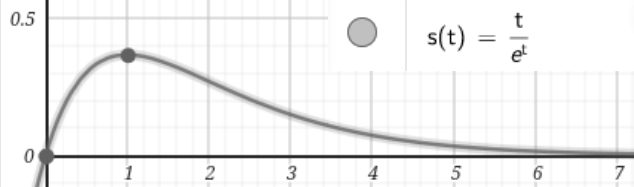
\includegraphics[width=0.6\textwidth]{../img/img_Lista3/3_s.png}
\end{figure}
\[v(t)=s'(t)= \frac{e^t-te^t}{e^{2t}}=\frac{e^t(1-t)}{e^{2t}}=\frac{1-t}{e^t}=(1-t)e^{-t}\]
\begin{figure}[H]
\centering
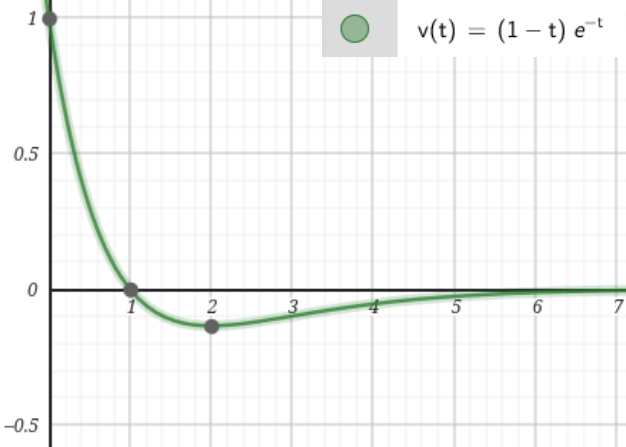
\includegraphics[width=0.6\textwidth]{../img/img_Lista3/3_v.png}
\end{figure}
\[a(t)=v'(t)= -(1-t)e^{-t}-e^{-t}=e^{-t}(-1+t-1)=(t-2)e^{-t}\]
\begin{figure}[H]
\centering
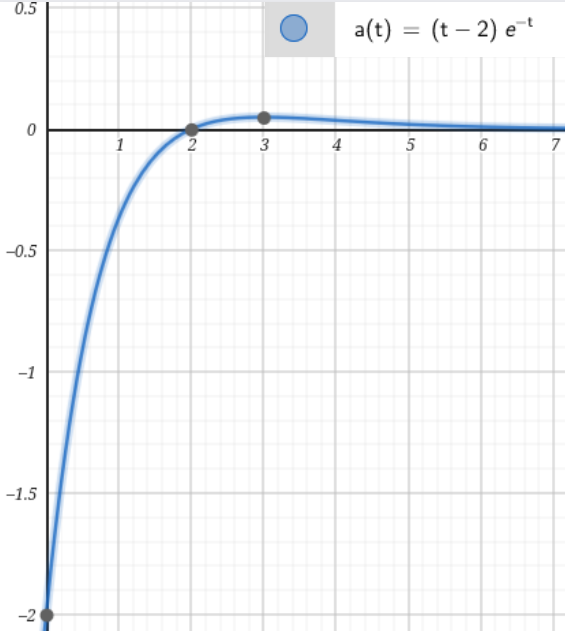
\includegraphics[width=0.5\textwidth]{../img/img_Lista3/3_a.png}
\end{figure}

\begin{enumerate}[label=(\alph*)]
\item Utilice la gráfica apropiada para hacer una estimación aproximada del momento en que la partícula invierte por primera vez la dirección de su movimiento; y luego encuentre la hora exacta.

  El análisis de signos de la función de velocidad en $v(t)$ muestra que la partícula se mueve en dirección positiva durante el intervalo de tiempo $0 \leq t < 1$, se detiene momentáneamente en el tiempo $t = 1$ y luego se mueve en la dirección negativa después de eso.
  
  $\therefore $ Cuando $v=0$ la partícula invierte por primera vez la dirección de su movimiento, en $t=1$.
  
\item Encuentre la posición exacta de la partícula cuando invierte por primera vez la dirección de su movimiento.

  En la gráfica de la función de la posición $s(t)$ en el momento $t = 1$ la partícula está en la posición $s = \frac{1}{e}$. En ese momento gira y viaja en dirección negativa.
  
\item Utilice las gráficas apropiadas para hacer una estimación aproximada de los intervalos de tiempo en los que la partícula se acelera y en los que se desacelera; y luego encuentre esos intervalos de tiempo exactamente.

  A partir de las gráficas de velocidad $v(t)$ y aceleración $a(t)$, podemos observar que durante el intervalo de tiempo $0<t<1$, la velocidad es positiva y la aceleración es negativa, por lo que la partícula se \textbf{desacelera}. Durante el intervalo de tiempo $1<t<2$ la velocidad y la aceleración son negativas, por lo que la partícula se \textbf{acelera}. Por último, durante el intervalo de tiempo $2<t$ la velocidad es negativa y la aceleración es positiva, por lo que la partícula se \textbf{desacelera}.
  
\end{enumerate}
    
% 40 -------------------------------------------------------------------------------------------------------------
\subsection{Ejercicio 40} Flores Morán Julieta Melina \\

Sean $s_A = 15t^2 + 10t + 20$ y $s_B = 5t^2 + 40t, t \geq 0$, las funciones de posición de los automóviles $A$ y $B$ que se mueven a lo largo de carriles rectos paralelos de una carretera.

\begin{enumerate}[label=(\alph*)]
\item ¿A qué distancia está el automóvil $A$ por delante del automóvil $B$ cuando $t = 0$?

  $s_A(0)-s_B(0)=20-0=20$
  
\item ¿En qué instantes de tiempo están los autos uno al lado del otro?
  \begin{align*}
    s_A(t)
    &=s_B(t)\\
    15t^2 + 10t + 20
    &= 5t^2 + 40t \\
    10t^2 -30t + 20
    &=0\\
    t^2 -3t + 2
    &=0\\
    (t-1)(t-2)
    &=0
  \end{align*}
  En el instante cuando $t=1$ o $t=2$.
  
\item ¿En qué instante de tiempo tienen la misma velocidad? ¿Qué coche va delante en este instante?
  \[
  v_A(t)=s_A'(t)=30t+10 \qquad v_B(t)=s_B'(t)=10t+40
  \]
  \begin{align*}
    v_A(t)
    &=v_B(t)\\
    30t+10
    &=10t+40\\
    20t
    &=30\\
    t
    &= \frac{3}{2} \\
    s_A(t)\vline_{t=\frac{3}{2}}
    &=15\left(\frac{3}{2}\right)^2 + 10\left(\frac{3}{2}\right) + 20 \\
    &= \frac{135}{4}+35 \\
    &= \frac{275}{4}\\
    s_B(t)\vline_{t=\frac{3}{2}}
    &= 5\left(\frac{3}{2}\right)^2 + 40\left(\frac{3}{2}\right) \\
    &= \frac{135}{4}+60 \\
    &= \frac{275}{4}\\
    &= \frac{45}{4}+60 \\
    &= \frac{285}{4}
  \end{align*}
  $\therefore $ Cuando $t=3/2$ tienen la misma velocidad y el automóvil $B$ está más adelante que el $A$.
\end{enumerate}

%%  -----------------------------------------------------------------------------------------------------------------------------------------------------------------------------------------------------------------------------
\section{Sección 4.7 \\ Método De Newton}
% 18 -------------------------------------------------------------------------------------------------------------
\subsection{Ejercicio 18} Zarco Romero José Antonio \\

Utilice una utilidad gráfica para determinar el número de veces que se cruzan las curvas; y luego aplique el método de Newton, cuando sea necesario, para aproximar las coordenadas $x$ de todas las intersecciones.
\[
y=\frac{1}{8}x^3-1 \qquad \text{ y } \qquad y=\cos{x}-2
\]
\begin{figure}[H]
\centering
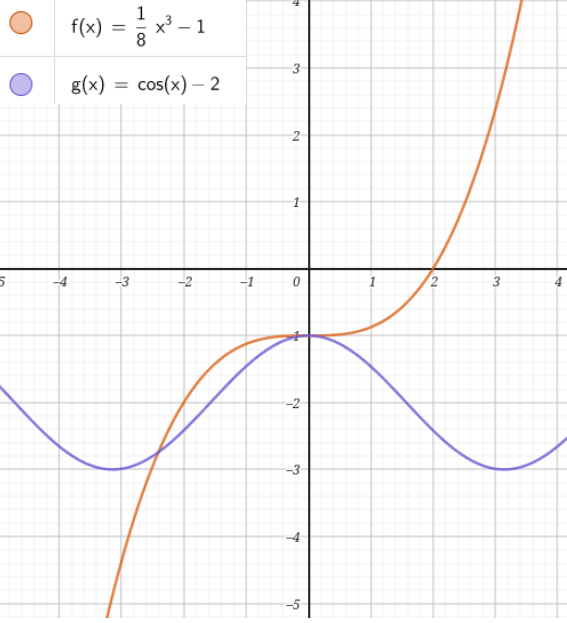
\includegraphics[width=0.6\textwidth]{../img/img_Lista3/newton18.png}
\end{figure}

Gracias a la gráfica de arriba podemos observar que $y=\frac{1}{8}x^3-1$ y $y=\cos{x}-2$ se intersectan  dos veces; en $x = 0$ y cerca de $x =-2$. \\

Primero, hay que reescribir la ecuación $\frac{1}{8}x^3-1=\cos{x}-2$ como
\begin{align*}
  \frac{1}{8}x^3-1-(\cos{x}-2)=0 \\
  \frac{1}{8}x^3-\cos{x}+1=0 
\end{align*}

De este modo, $f'(x)=\frac{3}{8}x^2+\sin{x}$. Juntando ambas ecuaciones, el método de Newton queda como
\[
x_{n+1} = x_n-\frac{\frac{1}{8}x_n^3-\cos{x_n}+1}{\frac{3}{8}x_n^2+\sin{x_n}}
\]

Usaremos $x_1=-2$ como nuestra primera aproximación. Así, sustituyendo el valor de $x_1$ y dejando $n = 1$, se obtiene
\[
x_2 = (-2)-\frac{\frac{1}{8}(-2)^3-\cos{(-2)}+1}{\frac{3}{8}(-2)^2+\sin{(-2)}} \approx -2.70449471
\]
A continuación, dejamos $n = 2$ y sustituimos $x_2$ para obtener
\[
x_3 = (x_2)-\frac{\frac{1}{8}(x_2)^3-\cos{(x_2)}+1}{\frac{3}{8}(x_2)^2+\sin{(x_2)}} \approx -2.46018026
\]

Si continuamos este proceso hasta que se generen dos aproximaciones idénticas en sucesión, obtenemos
\begin{align*}
  & x_1 = -2 \\
  & x_2 \approx -2.70449471 \\
  & x_3 \approx -2.46018026 \\
  & x_4 \approx -2.40859306 \\
  & x_5 \approx -2.40629828 \\
  & x_6 \approx -2.40629382 \\
  & x_7 \approx -2.40629382 \\
\end{align*}

% 34 -------------------------------------------------------------------------------------------------------------
\subsection{Ejercicio 34} Flores Morán Julieta Melina \\

Un \textit{\textbf{segmento}} de círculo es la región encerrada por un arco y su cuerda (Figura Ex-34). Si $r$ es el radio del círculo y $\theta$ el ángulo subtendido en el centro del círculo, entonces se puede demostrar que el área $A$ del segmento es $A = \frac{1}{2} r^2 (\theta - \sin{\theta})$, donde $\theta$ está en radianes. Encuentre el valor de $\theta$ para el cual el área del segmento es un cuarto del área del círculo. Calcula $\theta$ al grado más cercano.

\begin{figure}[H]
\centering
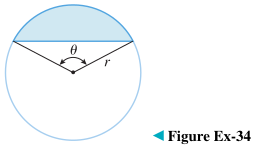
\includegraphics[width=0.5\textwidth]{../img/img_Lista3/3_34.png}
\end{figure}

En este caso hay que igualar las cantidades que queremos, el área de segmento y un cuarto del área del circulo que es $\pi r^2$. 
\[
 \frac{1}{2} r^2 (\theta - \sin{\theta}) = \frac{1}{4} \pi r^2
 \]
 E igualarla a 0 para buscar las soluciones, es decir, raíces que buscamos
 \[
 \frac{1}{2} r^2 (\theta - \sin{\theta}) = \frac{1}{4} \pi r^2
 \]
 \[
 r^2 (\theta - \sin{\theta}) = \frac{1}{2} \pi r^2
 \]
  \[
 \theta - \sin{\theta} = \frac{1}{2} \pi 
  \]
  \[
 \theta - \sin{\theta} - \frac{1}{2} \pi = 0
 \]
 Para aplicar la fórmula del método de Newton necesitamos la primera derivada de la funcioń que consideraremos $f(\theta) = \theta - \sin{\theta} - \frac{\pi}{2}$
 \begin{align*}
  f'(\theta)
  &= \frac{d}{d\theta} \left[  \theta - \sin{\theta} - \frac{\pi}{2} \right]\\
  &=   1 - \cos{\theta} 
 \end{align*}
 Ya con esta información aplicamos la fórmula dada:
 \[
 x_{n+1} = x_n - \frac{ \theta - \sin{\theta} - \frac{\pi}{2}}{ 1 - \cos{\theta} }
 \]
 Empezando de $\theta_1=2$\\
 $\theta_1 = 2$ \\
 $\theta_2 =  2 - \frac{ 2 - \sin{2} - \frac{\pi}{2}}{ 1 - \cos{2} }   = -2.339014106$ \\
 $\theta_3 =  2.339014106 - \frac{ 2.339014106 - \sin{2.339014106} - \frac{\pi}{2}}{ 1 - \cos{2.339014106} } = 2.310063197$ \\
 $\theta_4 =  2.310063197 - \frac{2.310063197 - \sin{2.310063197} - \frac{\pi}{2}}{ 1 - \cos{2.310063197} } = 2.309881467$ \\
 $\theta_5 =  2.309881467 - \frac{2.309881467 - \sin{2.310063197} - \frac{\pi}{2}}{ 1 - \cos{2.309881467} } = 2.30988146$ \\
 $\theta_6 =  2.30988146 - \frac{2.30988146 - \sin{2.30988146} - \frac{\pi}{2}}{ 1 - \cos{2.30988146} } = 2.30988146$ \\

 Después de este valor se aproximan a más de 10 decimales.
\end{document}
